\documentclass[12pt,a4paper]{article}
\setcounter{tocdepth}{4}
\usepackage[left=3cm,right=3cm,top=3cm,bottom=3cm]{geometry}
\usepackage{graphicx}
\usepackage{subcaption}
\usepackage{float}
\graphicspath{ {./images/} }

\begin{document}

    \begin{titlepage}
        \centering
        \title{COMP3419 Assignment 1\thanks{Option 1}}
        \author{Nick Zhou 460363707}
        \date{October 2018}
        \maketitle
        \centering
        
\includegraphics[width=4cm]{usyd}\\[2cm]
    \end{titlepage}

    \begin{tableofcontents}
        \tableofcontents
    \end{tableofcontents}

    \section{Introduction}

      \subsection{Preamble}

      The purpose of this report is to demonstrate the pipeline used to complete the COMP3419 Assignment (Option 1). This report consists of\
      a three main sections, introduction, implementation and conclusion. This report was created with \LaTeX{} as required by the assignment\
      specification.\\

      \subsection{Task}

      The task of this assignment was to program a short video involving digital video processing, compositing and 2D animation techniques.\
      The output is a piece of animation based on the provided clip. The video was of a marionette monkey with red markers on the head, hands\
      abd feet. Our task invovled tracking these red markets in order to determine the motion of the marionette monkey and recreate it with\
      our own character. The programming language used to complete this assignment was python3 on the windows operating system.\\

      In summary this assignment task was broken into a set of 4  subtasks excluding this report:
      \begin{itemize}
        \item \textbf{Motion Capture}: The body of the monkey is labelled with red markets. The subtask involved segmenting the red markers in order to\
        track the motions of the monkey.
        \item \textbf{Replace Background and Marionette}: The blue background was to be replaced with a dynamic background. The monkey marionette was to\
        be replaced with our own character with the original motions of the old marionette being preserved.
        \item \textbf{Intelligent Objects}: Two randomly moving must be added to the video and interact with the marionette in at least two different ways.\
        Special effects were to be triggered when interactions between the marionette and intelligent object occurs.
        \item \textbf{Sound Track}: At least two sound tracks must be added to the video. The sound track should relate to the interaction between\
        the intelligent objects and the marionette.
      \end{itemize}

    \section{Implementation}
    The red parts of the monkey were found by first converting the frames to HSV (Hue Saturation Value) and then applying a threshold. The\
    use of HSV to threshold the red parts of the monkey proved to be far superior to using RGB. The segmentation of the red markersr was\
    enhanced by performing two iterations of morphological erosion operations followed by a single iteration dilation operation and finally\
    another iteration of erosion. An elliptical structuring element of was used to perform these morphological operations.

      \subsection{Algorithm}
      The K-Medoids algorithm was used to discern the the red dots into proper clusters to identify each part of the monkey. Those parts being\
      the head, two arms and two legs. The initial centers of the clusters were manually set to be as close to the middle of each of the monkey\
      parts as possible.

      \subsection{Experimental Results}
      In trying to find the red dots on the monkey, various morphological techniques were used. Performing a closing operating resulted in the\
      "clusters" that had very low dissimilarity.
      \\

      An opening operation yielded a result where the 5 red markers were more easy to discern and very dissimilar to each other.
      \\

      Various other operations such as alternating between erosion and dilation operations with different number of itereations were performed.\
      Eroding for more than 2 iterations before performing a dilation resulted in too few red pixels being retained. If dilating was performed first,\
      the red dots joined too close to each other. This resulted in poorer cluster centers.
      \\

      Various structuring elements were used when experimenting with the morophological operations. A square structuring element was found to...

    \section{Conclusion}

    The implementation of k-medoids was very susceptible to noise. Fast movements would often results in the clusters being messed up.\
    The cross over of the two legs markers resulted did not break the clustering algorithm in matching the motions of the monkey. The\
    heavy amount of erosion performed on the image prevented the two clusters from forming a single one.

      \subsection{Motion Capture}

      Despite the many draw backs of the implementation, all four tasks required for the assignment were certainly met successfully.\
      Most of the motions of the monkey were accurately captured using the K-Medoids classifier.

      \subsection{Background and Marionette Replacement}

      The blue background and the monkey was replaced as required by the specification. The character replacement (Donald Trump) simulated the gestures of the monkey and\
      had all 5 connected components.

      \begin{figure}[H]
        \includegraphics[width=8cm]{original}
        \caption{This still shows a frame of the original video with the blue background and monkey marionette}
      \end{figure}
      \begin{figure}[H]
        \includegraphics[width=8cm]{replaced}
        \caption{This still shows a frame of the output video in which the background and marionette is replaced}
      \end{figure}


      \subsection{Intelligent Objects}

      The condition of having two intelligent objects interact with the marionette was met and their\
      motions were certainly affected when they came into contact with each other. A requirement of a special effect being trigged\
      when iteractions happen was satisfied as demonstrated in figure 1.

      \begin{figure}[H]
        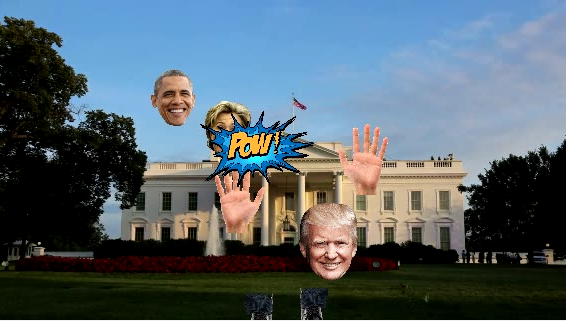
\includegraphics[width=8cm]{pow}
        \caption{A still image of a special effect being triggered when an intelligent object collides with the marionette}
      \end{figure}

      \subsection{Sound Track}

      Two soundtracks were programmed for the video. They are triggered to play when the intelligent objects colllide with the marionette.\
      The sound track that is played depends on the type of intelligent object that collides with the marionette. If it is an Obama object,\
      the sound track "you're fired" is played. Alternatively, when a Hillary object collides with the marionette, the "such a nasty woman"\
      sound track is played.


        \begin{figure}[H]
          \centering
          \begin{subfigure}[H]{0.32\textwidth}
            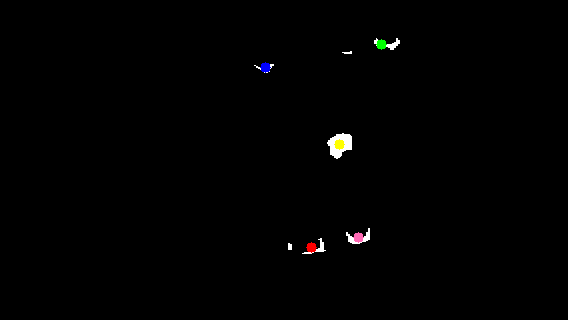
\includegraphics[width=\linewidth]{192}
            \caption{frame 1}
          \end{subfigure}
          \begin{subfigure}[H]{0.32\textwidth}
            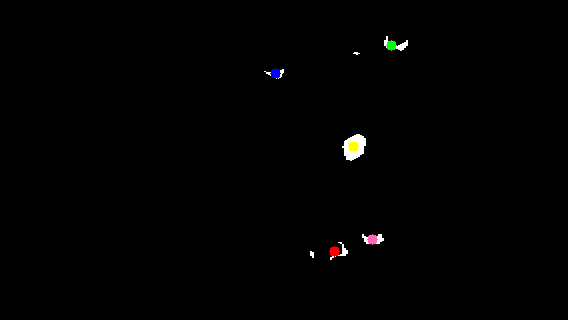
\includegraphics[width=\linewidth]{193}
            \caption{frame 2}
          \end{subfigure}
          \begin{subfigure}[H]{0.32\textwidth}
            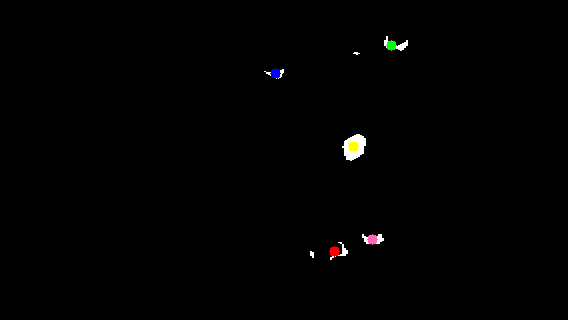
\includegraphics[width=\linewidth]{193}
            \caption{frame 3}
          \end{subfigure}
          \begin{subfigure}[H]{0.32\textwidth}
            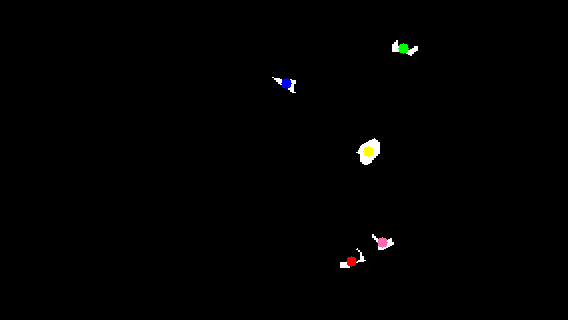
\includegraphics[width=\linewidth]{194}
            \caption{frame 4}
          \end{subfigure}
          \begin{subfigure}[H]{0.32\textwidth}
            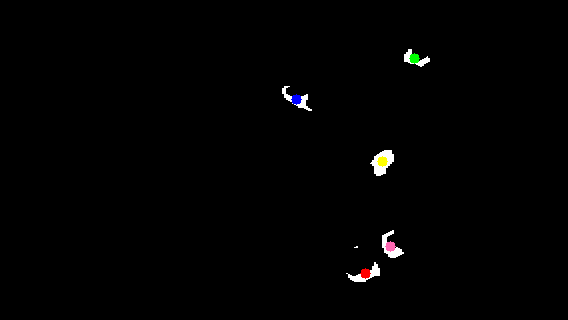
\includegraphics[width=\linewidth]{195}
            \caption{frame 5}
          \end{subfigure}
          \begin{subfigure}[H]{0.32\textwidth}
            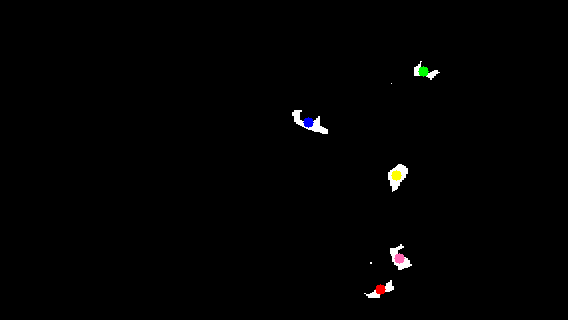
\includegraphics[width=\linewidth]{196}
            \caption{frame 6}
          \end{subfigure}

          \caption{Example of the marked centers being accurate over a series of moving frames}
        \end{figure}
        \
        \begin{figure}[H]
          \centering
          \begin{subfigure}[H]{0.49\textwidth}
            \includegraphics[width=\linewidth]{883}
            \caption{Example of the clusters being misidentified due to noise}
          \end{subfigure}
          \begin{subfigure}[H]{0.49\textwidth}
            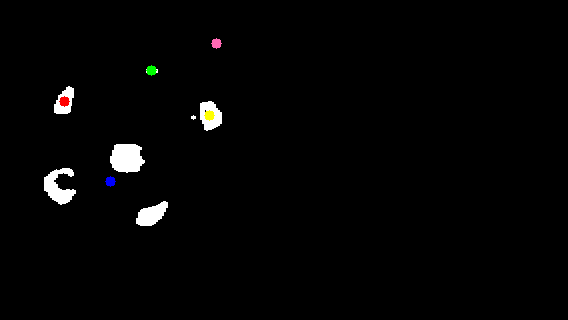
\includegraphics[width=\linewidth]{952}
            \caption{As a result of the cluster centroids being misidentified in previous frames such as the previous figure, the initial medoids result in incorrect classification of the monkey parts}
          \end{subfigure}
        \caption{When the clusters start being misclassified, future frames will also be misclassified}
        \end{figure}


    \listoffigures
\end{document}
